% !TEX TS-program = lualatex

% required for TexXstudio, an alternative is to change the default bibliography tool 
% in TeXstudio settings (Options > Configure TeXstudio > Build > Default Bibliography Tool)
% !BIB TS-program = biber

\documentclass[a4paper,11pt]{article}

\usepackage{geometry}
\geometry{left=20.00mm, right=15.00mm, top=20.00mm, bottom=20.00mm}

% this is to get rid of 'Overfull \hbox...' errors
\usepackage{microtype}

% ------------------------------------------------------------------------------
% Title
% ------------------------------------------------------------------------------

\title{\vspace{-1.5cm}Математический анализ и линейная алгебра \\
Домашнее задание №1}
\author{Дмитрий Донецков (ddonetskov@gmail.com)}
\date{\today}

% ------------------------------------------------------------------------------
% LUA
% ------------------------------------------------------------------------------

% \usepackage{luacode}

% ------------------------------------------------------------------------------
% Graphics
% ------------------------------------------------------------------------------

\usepackage{graphicx}

% ------------------------------------------------------------------------------
% Figures
% ------------------------------------------------------------------------------

\usepackage{subcaption}         % subcaptions in figures

% ------------------------------------------------------------------------------
% Tables
% ------------------------------------------------------------------------------

\usepackage{multirow}           % spanning columns across multiple rows
\usepackage{makecell}           % allows different formats inside cells

\renewcommand\theadalign{bc}
\renewcommand\theadfont{\bfseries}
\renewcommand\theadgape{\Gape[4pt]}
\renewcommand\cellgape{\Gape[4pt]}

% ------------------------------------------------------------------------------
% Math (Additional Support)
% ------------------------------------------------------------------------------

\usepackage{amsmath,amsfonts,amssymb,amsthm,mathtools}     % AMS
\usepackage{cancel}             % four different modes of striking through
\usepackage{dsfont}
\usepackage{icomma}             % Smart comma: $0,2$ --- число, $0, 2$ --- перечисление
\usepackage{nicefrac}
\usepackage{physics}            % implementation of \abs and \norm

\DeclareMathOperator*{\D}{\mathbb{D}}   % the dispersion symbol
\DeclareMathOperator*{\E}{\mathbb{E}}   % the expectation symbol
\DeclareMathOperator*{\N}{\mathbb{N}}   % the set of natural numbers
\DeclareMathOperator*{\R}{\mathbb{R}}   % the set of real numbers
\DeclareMathOperator*{\Z}{\mathbb{Z}}   % the set of integers

% ------------------------------------------------------------------------------
% Russian Language (support thereof)
% ------------------------------------------------------------------------------

\usepackage[russian,english]{babel}	    % локализация и переносы

% ------------------------------------------------------------------------------
% Fonts 
% ------------------------------------------------------------------------------

\usepackage{fontspec}           % required to load Open Type, True Type fonts

\setmainfont{CMU Serif}
\setsansfont{CMU Sans Serif}
\setmonofont{CMU Typewriter Text}

%\setmainfont{Linux Libertine O} % Libertine covers Latin, Hebrew, Greek, and Russian
%\setmonofont{Courier New}

\usepackage{euscript}	          % Шрифт Евклид
\usepackage{mathrsfs}           % Красивый матшрифт

% ------------------------------------------------------------------------------
% Bibliography 
% ------------------------------------------------------------------------------

% Removed as it was not required.

% ------------------------------------------------------------------------------
% Bookmarking, citing, URL's
% ------------------------------------------------------------------------------

% hyperref usually needs to be loaded last
\usepackage{hyperref}
\usepackage{url}
\usepackage[dvipsnames]{xcolor}

\hypersetup{
    colorlinks=true,
    linkcolor=blue,
    filecolor=red,      
    urlcolor=blue,
}

\urlstyle{same}

\begin{document}

\maketitle

\section{Задача 1}

Графики заданных функций \textit{a-f} отображены на рис. \ref{fig:task1}.

\begin{figure}[h!]
  \centering
    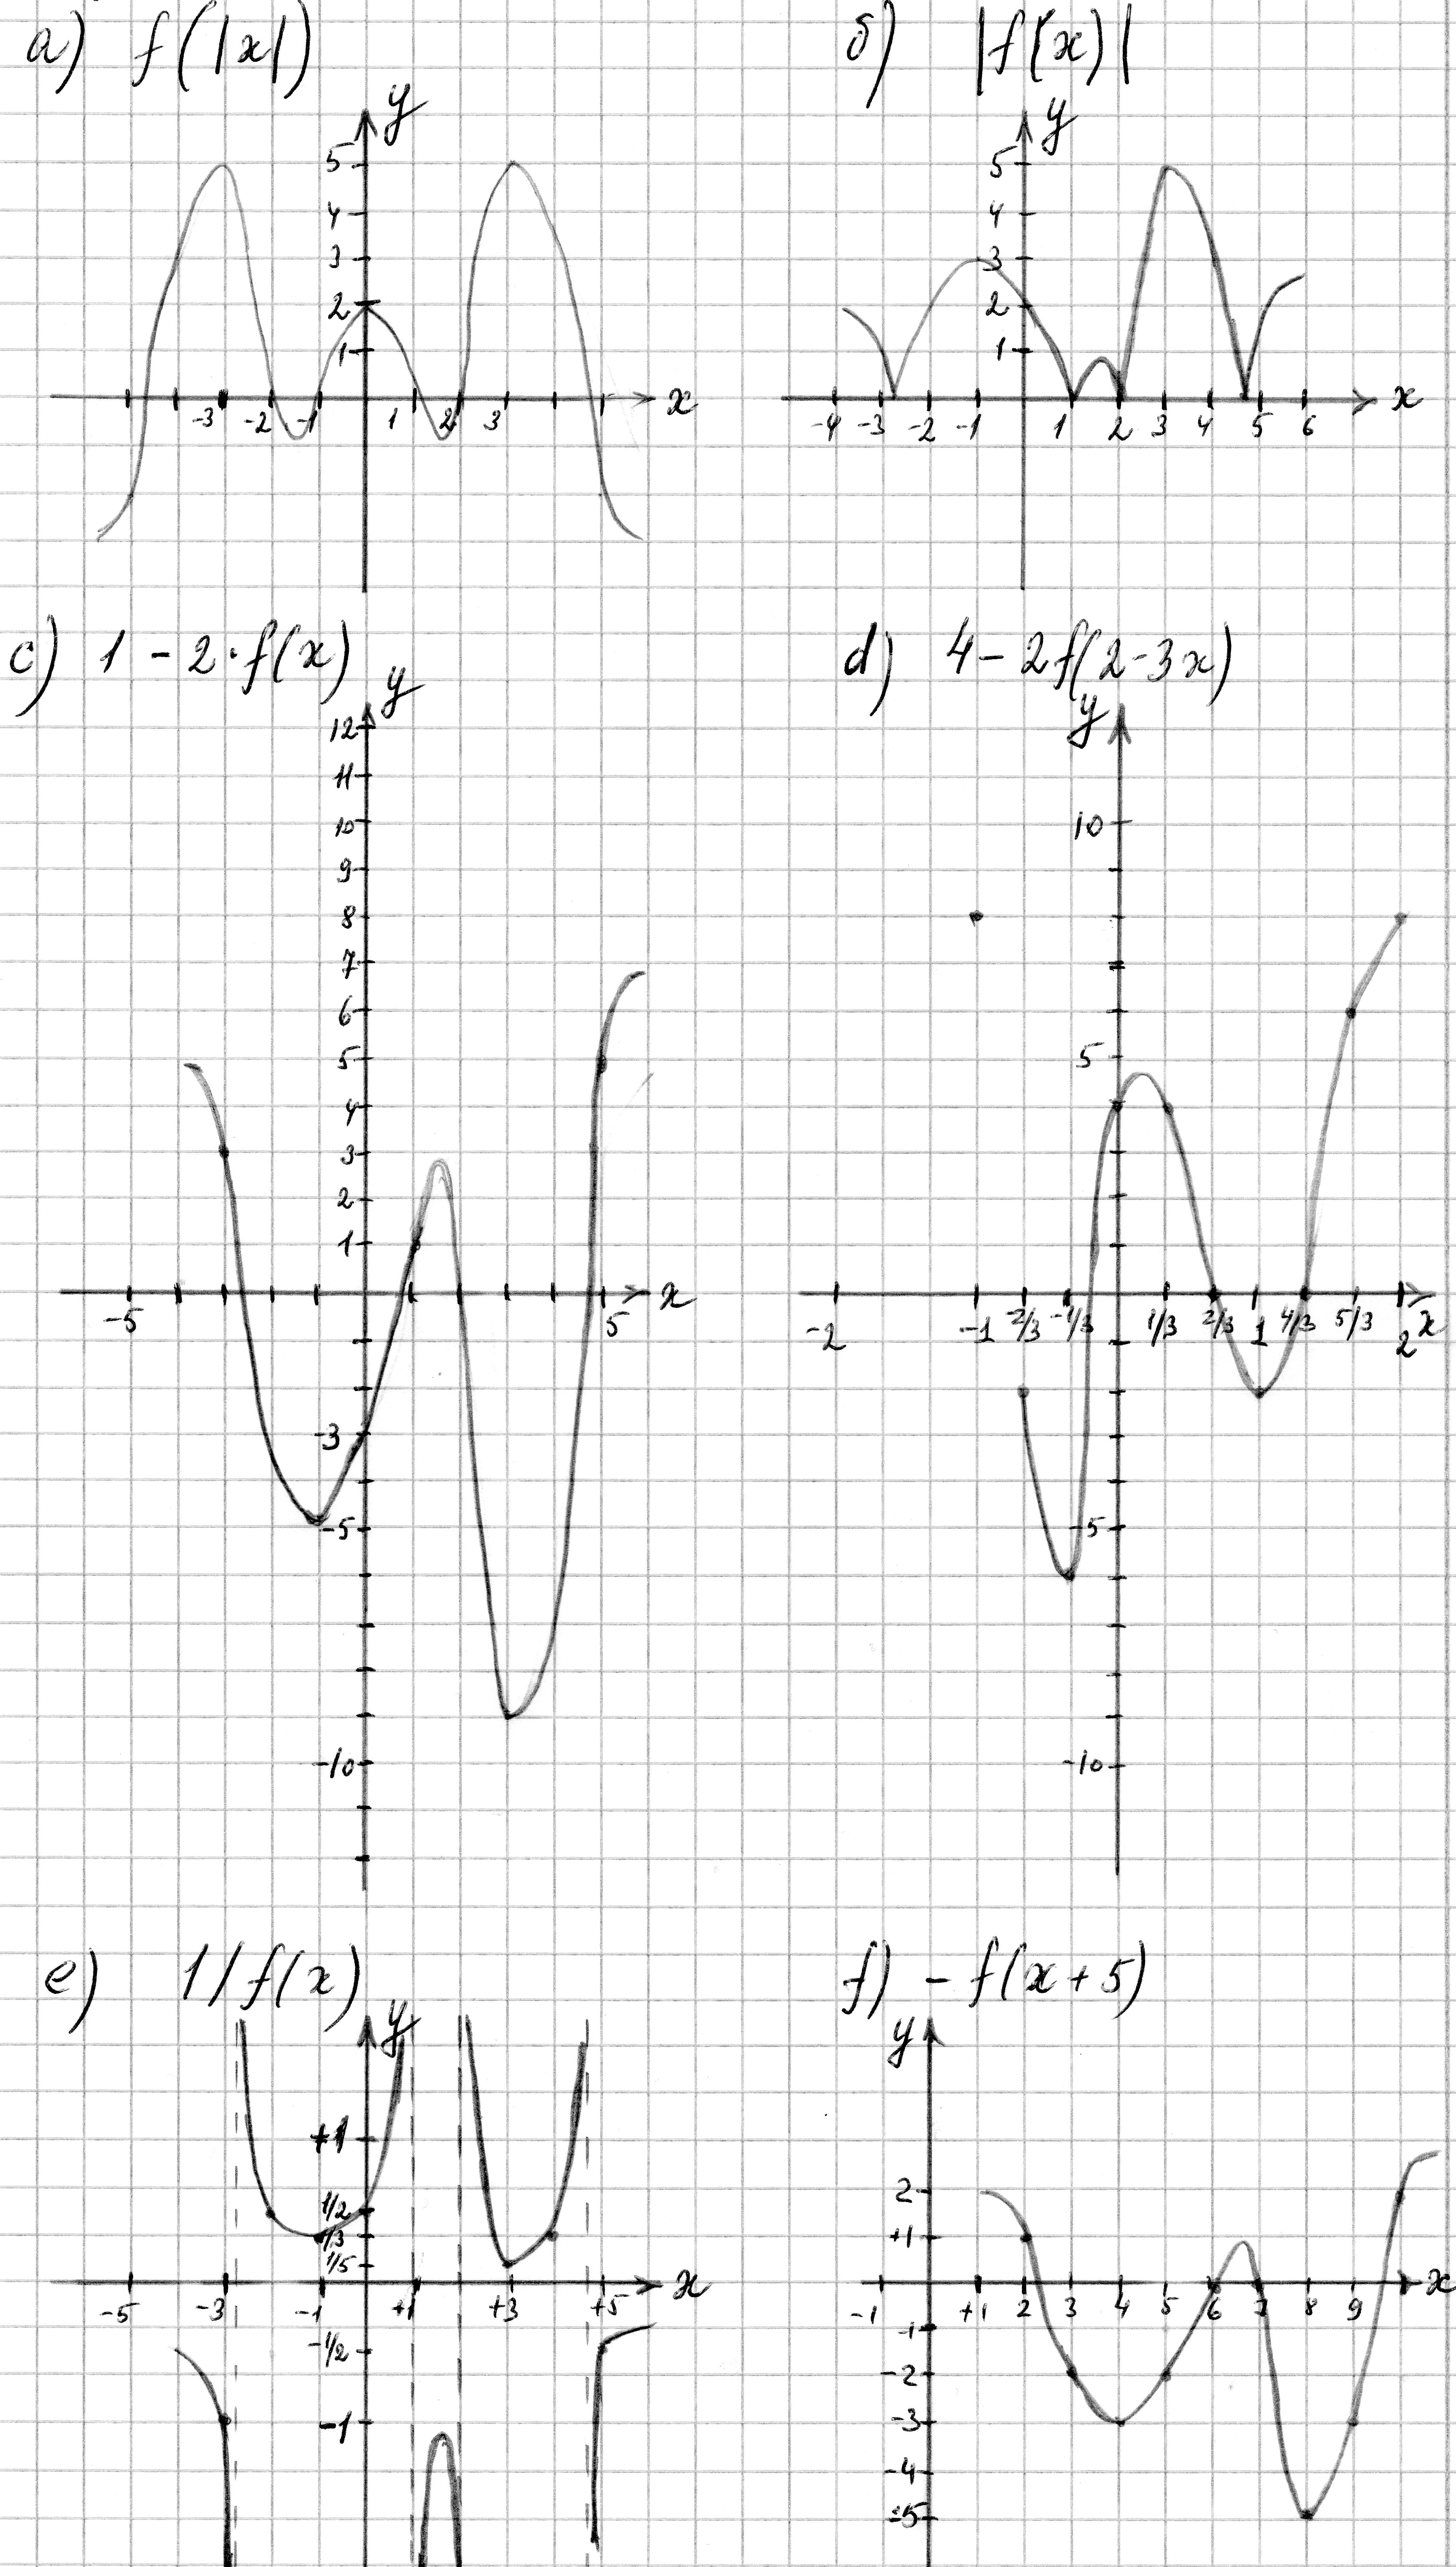
\includegraphics[height=18cm]{images/task1.jpg}
  \caption{Графики функций (задача 1)}
  \label{fig:task1}
\end{figure}

\section{Задача 2}

Заданную функцию можно представить в виде набора интервальных функций:

\begin{equation}
  \label{eq:task2}
f(x) = \frac{(x+1)(x-1)}{\abs{x-1}} = 
  \begin{cases}
    \frac{(x+1)(x-1)}{-(x-1)}, & \text{если}\ x<1 \\
    \frac{(x+1)(x-1)}{{x-1}}, & \text{если}\ x>1 \\
    \text{не определена}, & \text{если}\ x=1
  \end{cases}
  = 
  \begin{cases}
   -(x+1), & \text{если}\ x<1 \\
     x+1,  & \text{если}\ x>1 \\
    \text{не определена}, & \text{если}\ x=1.
  \end{cases}
\end{equation}

Тогда, график функции будет выглядеть следующим образом: см. рис. \ref{fig:task2}.

\begin{figure}[h]
  \centering
    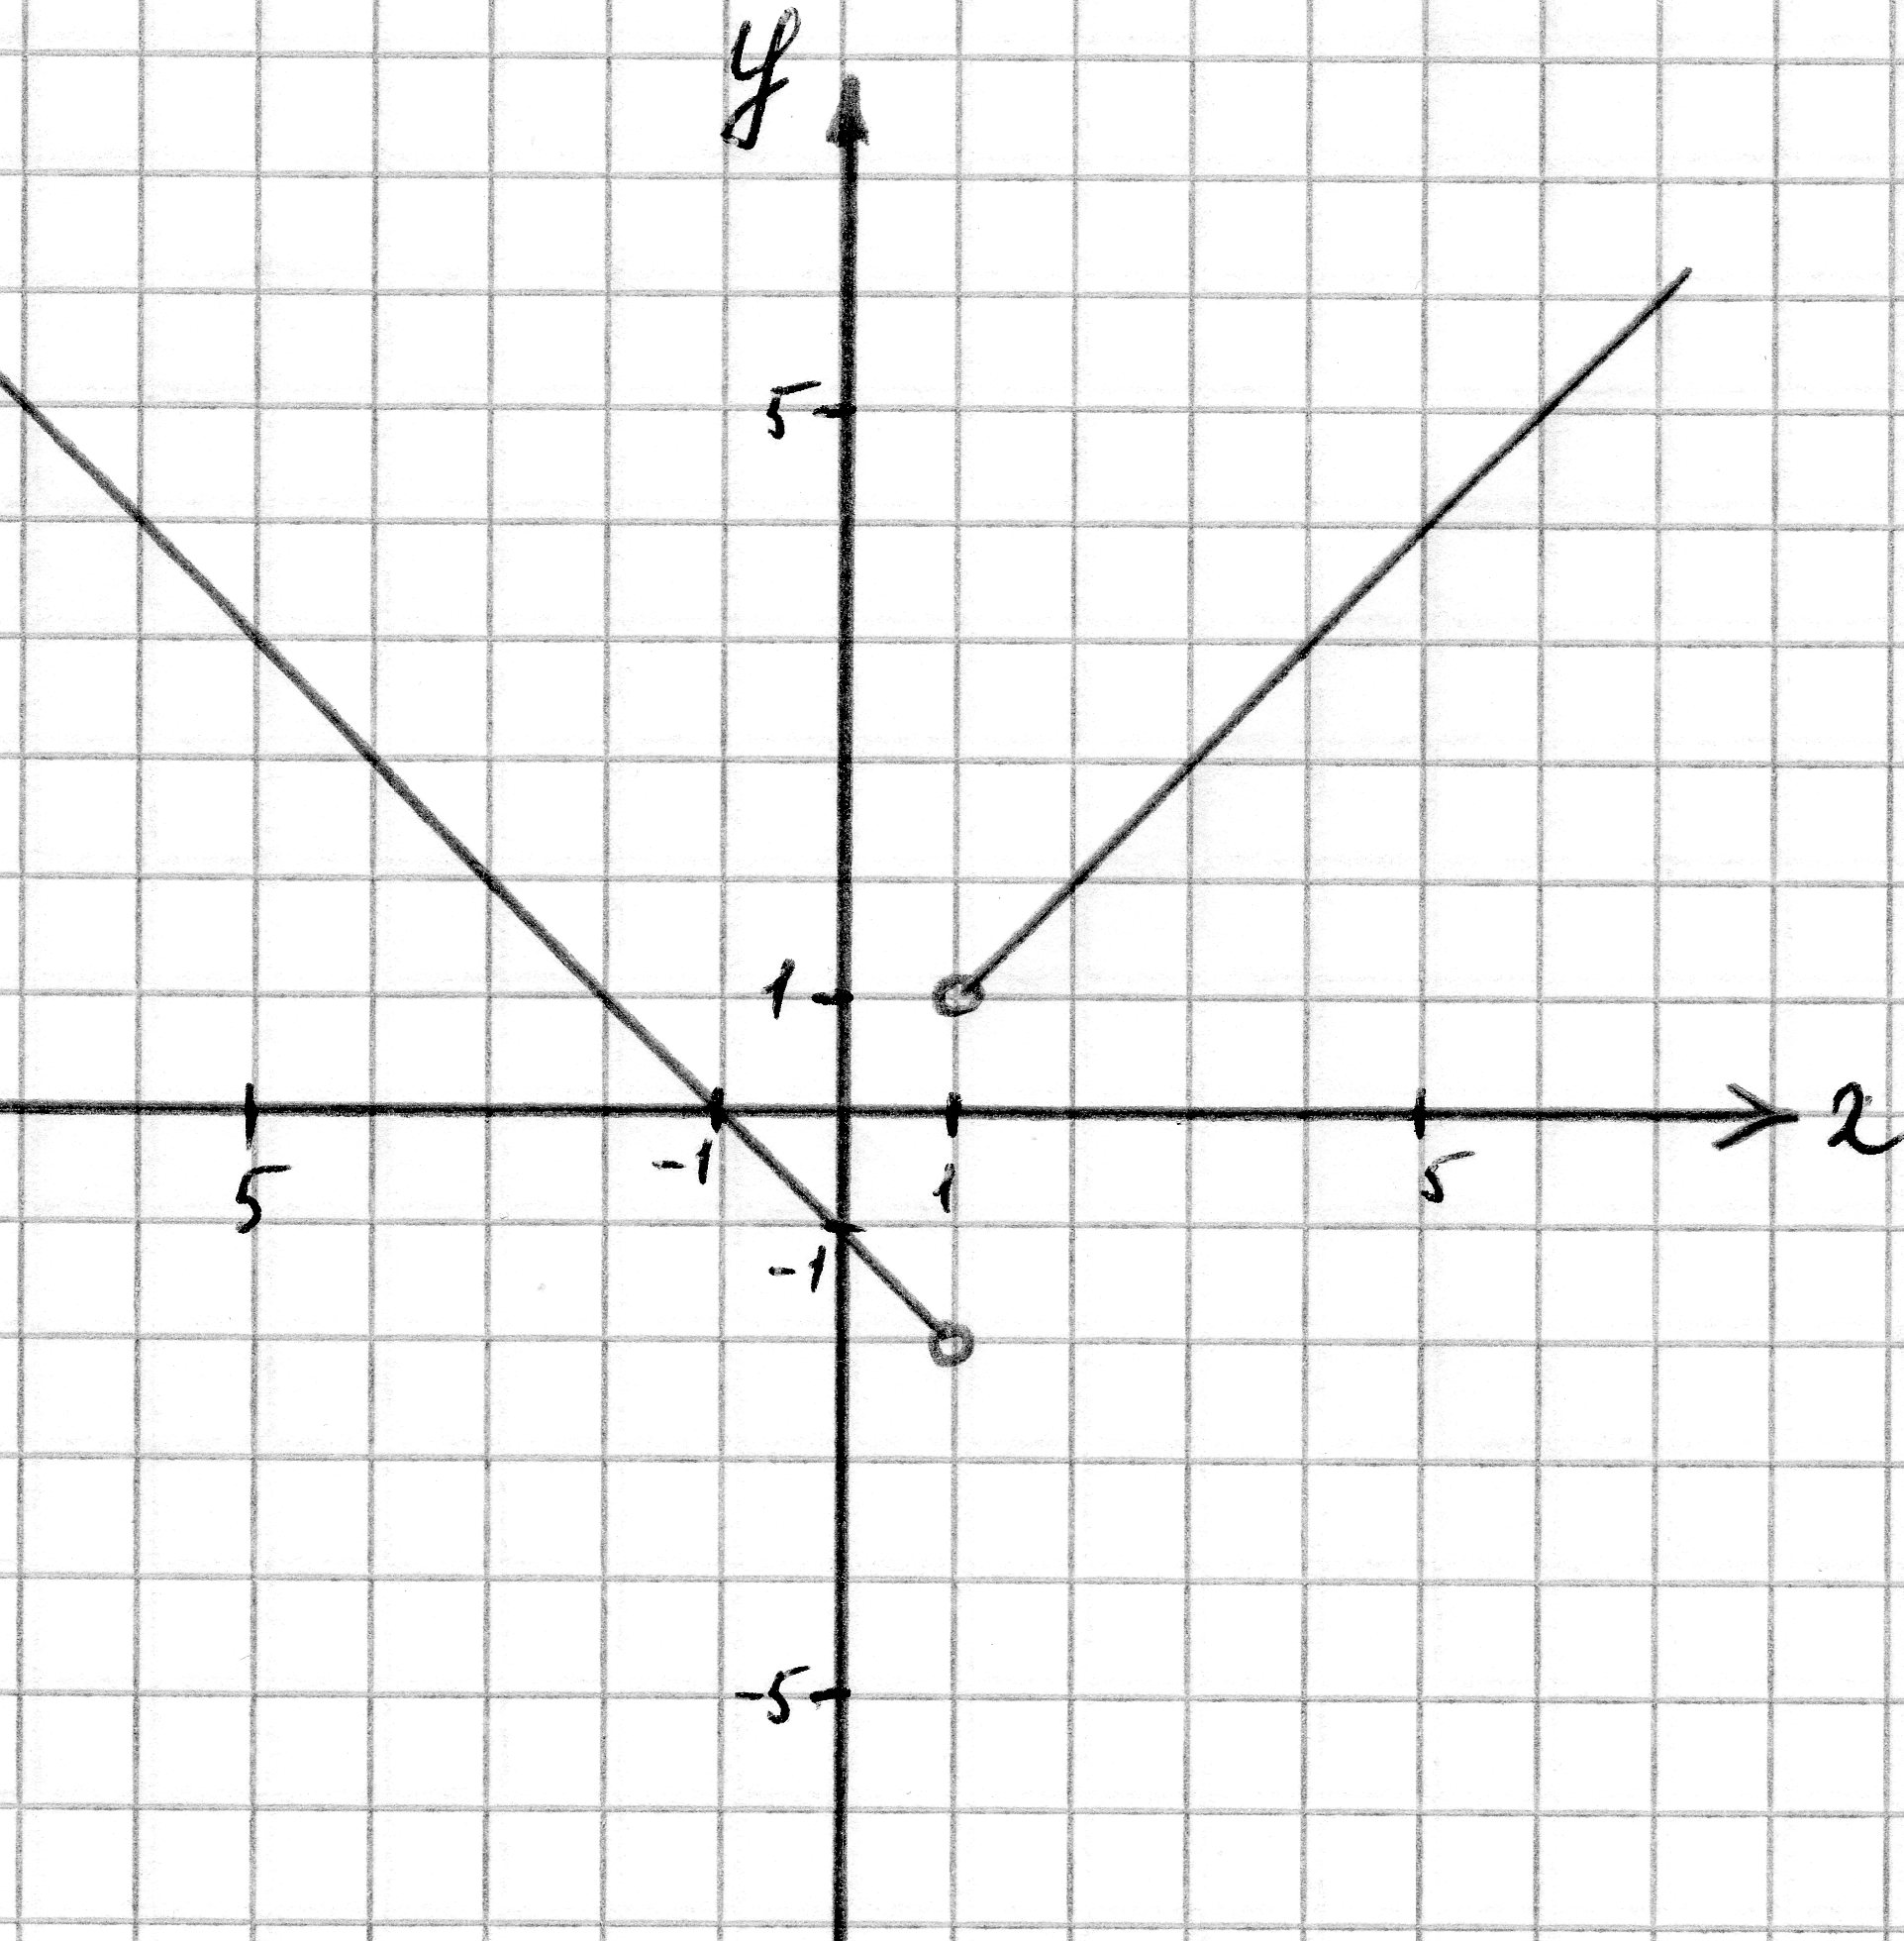
\includegraphics{images/task2.jpg}
  \caption{График функции (задача 2)}
  \label{fig:task2}
\end{figure}

Искомые пределы согласно выражению \ref{eq:task2}:

\begin{equation*}
\begin{split}
\lim_{x \rightarrow 1^+} f(x) & = \lim_{x \rightarrow 1^+} x+1 = 2. \\
\lim_{x \rightarrow 1^-} f(x) & = \lim_{x \rightarrow 1^-} -(x+1) = -2. \\
\lim_{x \rightarrow 1}   f(x) & \Rightarrow \text{предел не существует}.
\end{split}
\end{equation*}

\section{Задача 3}

\begin{itemize}
\item Функция $f^{-1}$ \textbf{не существует}, т.к. нет однозначного обратного отображения: из области значений функции $f$  в область её определения, например, для значения $f=4$ нет такого однозначного обратного отображения.
\item Функция $f \circ g = f(g(x))$ \textbf{существует}, т.к. для всей области значений функции $g$ определено отображение в область значений функции $f$, таблица для $f(g(x))$ указана ниже, областью определения для неё являются все указанные значения $x$, а областью отражения - все указанные значения $f(g(x))$.

\begin{tabular}{|c|c|c|c|c|c|c|c|}
\hline 
 $x$       & 1 & 2 & 3 & 4 & 5 & 6 & 7 \\ 
\hline 
 $g(x)$    & 7 & 6 & 1 & 2 & 3 & 4 & 5 \\ 
\hline 
 $f(g(x))$ & 0 & 6 & 4 & 8 & -1 & 4 & 7 \\
\hline 
\end{tabular} 

\item Функция $g \circ f = g(f(x))$ \textbf{не существует}, т.к. не для всей области значений функции $f$ определено отображение в область значений функции $g$.
\item Функция $f \circ f = f(f(x))$ \textbf{не существует}, т.к. не для всей области значений функции $f$ определено отображение в область значений той же самой функции $f$.
\end{itemize}

\section{Задача 4}

Функция $f(x)$ задана тремя элементарными функциями на трех интервалах, параметры $a$, $b$ следует выбрать такими, чтобы функция была непрерывной на всей области определения $x \in (-\infty,+\infty)$, включая границы между интервалами. Для заданных интервалов, без рассмотрения границ самих интервал, функция $f(x)$ уже непрерывна, т.к. заданные элементарные функции непрерывны на них.

Тогда нам следует найти такие значения параметров $a$, $b$, чтобы

\begin{equation*}
  \begin{cases}
    \lim_{x \rightarrow 0} ax + b & = \lim_{x \rightarrow 0} e^2 \\
    \lim_{x \rightarrow 2} ax + b & = \lim_{x \rightarrow 2} x^2 - 3
  \end{cases}
  \Rightarrow
  \begin{cases}
    \lim_{x \rightarrow 0} ax + b & = e^2 \\
    \lim_{x \rightarrow 2} ax + b & = 1
  \end{cases}
  \Rightarrow
    a = \frac{1-e^2}{2}, b = e^2.
\end{equation*}

\section{Задача 5}

Данное уравнение можно представить в виде функции $f(x) = 100 e^{\nicefrac{-x}{100}} - 0.01x^2$. Тогда, для доказательства того, что уравнение имеет хотя бы один вещественный корень, необходимо доказать, что функция $f(x)$: а) непрерывна, б) меняет знаки для каких-нибудь двух значений.

Функция непрерывна, т.к. составляющие её элементарные функции непрерывны для всех $x \in (-\infty,+\infty)$.

Проверим на случаи смены знаков на примере некоторых значений $x$:

\begin{equation}
  \label{eq:task5}
  \begin{split}
  \text{если}\ x & = 100, \text{то}\  f(x) = 100e^{-1} - 100 < 0 \\
  \text{если}\ x & = -100, \text{то}\ f(x) = 100e - 100 > 0
  \end{split}
\end{equation}

Исходя из выражения \ref{eq:task5}, согласно теореме о промежуточном значении функция должна принимать значение равным нулю на интервале $x \in (-100,+100)$, что означает, что уравнение имеет корень на данном интервале.

\section{Задача 6}

Найдём производную заданной функции:

\begin{equation*}
f'(x) = \frac{2(x+1) - 2x}{(x+1)^2} = \frac{2}{(x+1)^2}.
\end{equation*}

Тогда согласно уравнению касательной к функции в заданной точке $(x_0, y_0) = (1, 1)$, искомое уравнение касательной:

\begin{equation*}
y - f(y_0) = f'(x_0)(x - x_0) \Rightarrow y - 1 = \frac{1}{2}(x-1) \Rightarrow y = \frac{1}{2}(x+1).
\end{equation*}

\section{Задача 7}

\begin{equation*}
\begin{split}
(\cos(\sin x^2))' & = (\sin x^2)'\cos'(\sin x^2) = (x^2)' \sin' x^2 \cos'(\sin x^2) \\
& = 2x \cos x^2 (-\sin (\sin x^2)) = - 2x \cos x^2 \sin (\sin x^2).
\end{split}
\end{equation*}

\begin{equation*}
\begin{split}
(\cos(\sin^2 x))' & = (\cos(\sin x \sin x))' = (\sin x \sin x)' \cos' (\sin x \sin x)) \\
& = (\sin' x \sin x + \sin x \sin' x) \cos' (\sin x \sin x)) = - (\cos x \sin x + \sin x \cos x) \sin (\sin^2 x) \\
& = -2 \sin x \cos x \sin (\sin^2 x).
\end{split}
\end{equation*}

\section{Задача 8}

Найдём первую и вторую производные $f(x)$:

\begin{equation*}
\label{eq:task8_der1}
f'(x)  = \cos' x \ln'(\cos x) = -\sin x \frac{1}{\cos x} = -\frac{\sin x}{\cos x}. \\
\end{equation*}

\begin{equation*}
\label{eq:task8_der2}
f''(x) = -1 \frac{\sin' x \cos x - \cos' x \sin x}{\cos^2 x} = -\frac{\cos^2 x + \sin^2 x}{\cos^2 x} = -1 - (\frac{\sin x}{\cos x})^2.
\end{equation*}

Первая производная $f'(x)$ принимает значение ноль при $x = n \pi, n \in \Z$, вторая производная $f''(x)$ при данных значениях $x$ всегда принимает значения меньше нуля. Соответственно, это точки локальных максимумов функции. Точек локальных минимумов у функции нет.

Рассмотрим знаки первой производной $f'(x)$ на интервале периодичности составляющих её элементарных функций $x \in [0, 2\pi]$:

\begin{equation*}
  f'(x) = 
  \begin{cases}
    \geq 0, & x \in [0, \frac{\pi}{2}) \\
    < 0, & x \in (\frac{\pi}{2}, \pi) \\
    \geq 0, & x \in [\pi, \frac{3}{2}\pi) \\
    \leq 0, & x \in (\frac{3}{2}\pi, 2\pi]
  \end{cases}
\end{equation*}

Обобщая для всего множества $\R$, функция $f(x)$ растёт при $x \in [n \pi, n \pi + \frac{\pi}{2}), n \in \Z$ и убывает при $x \in (n \pi - \frac{\pi}{2}, n \pi], n \in \Z$.

% ------------------------------------------------------------------------------
% Bibliography
% Is that possible to make it as per ГОСТ Р7.05-2008?
% ------------------------------------------------------------------------------
%\printbibliography[heading=bibintoc,title={References}]

\end{document}
